\begin{figure*}[p]
	\vspace{-1em}
	\centering
	\begin{tabular}{ccc}
		\subfloat[][\sf ais2klinik]{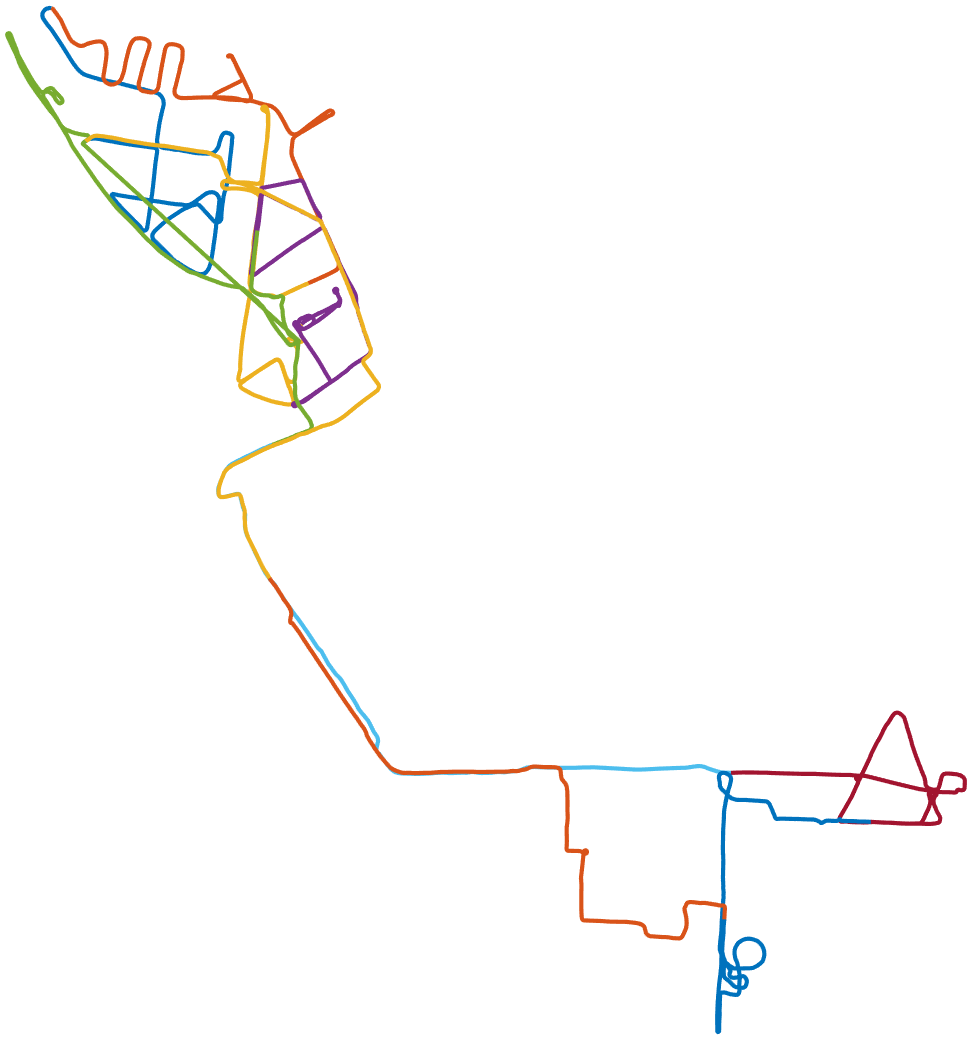
\includegraphics[trim =0mm 0mm 0mm 0mm,width=0.25\textwidth]{figures/benchmark/ais2klinik.png}} &
		\hspace{1em}\subfloat[][\sf city]{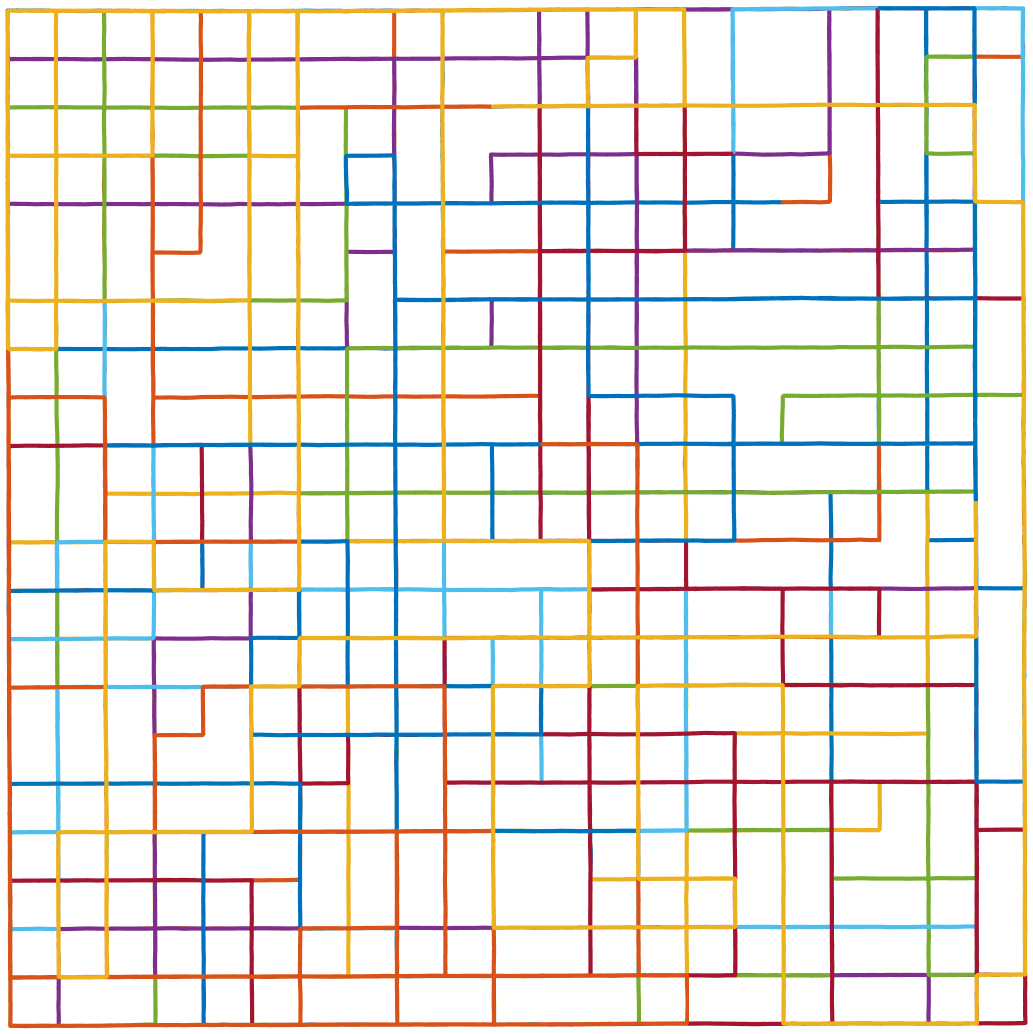
\includegraphics[trim =0mm 0mm 0mm 0mm,width=0.25\textwidth]{figures/benchmark/city10000.png}} &
		\hspace{1em}\subfloat[][\sf CSAIL]{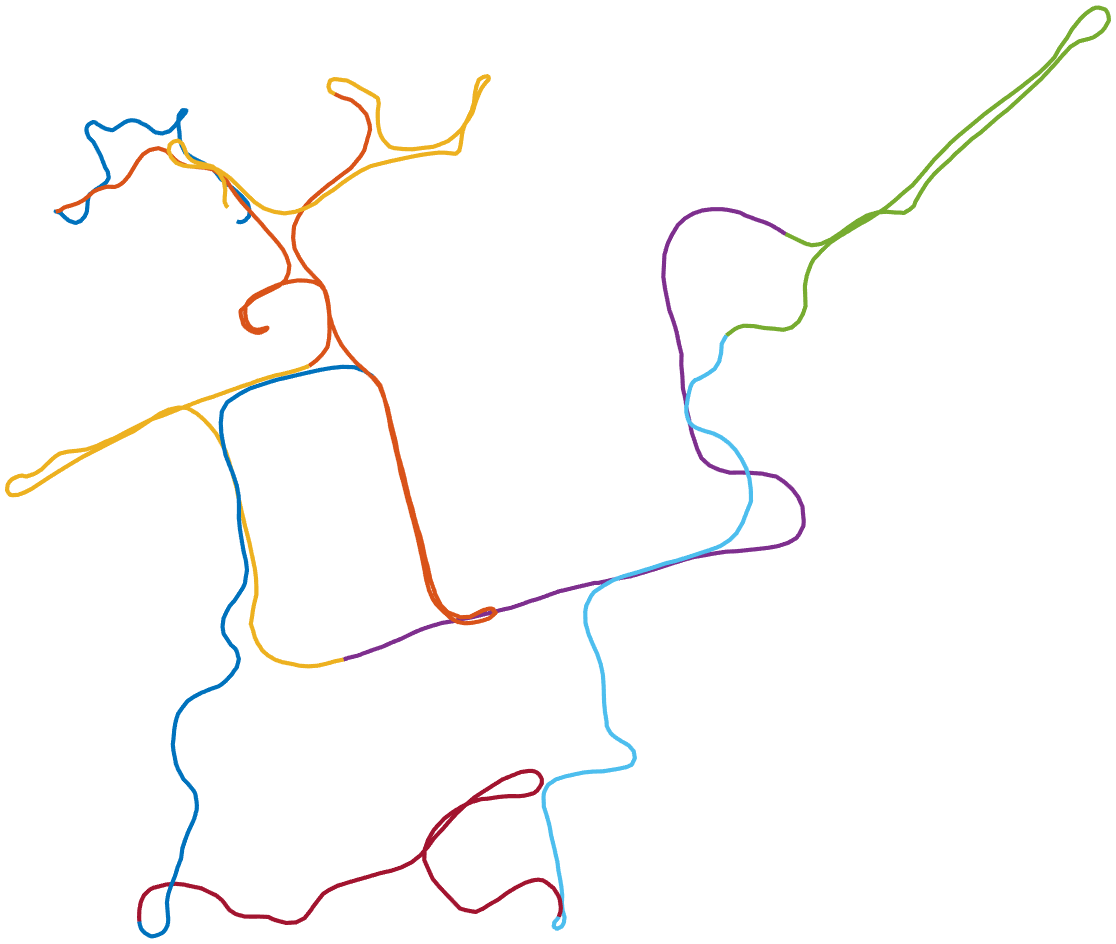
\includegraphics[trim =0mm 0mm 0mm 0mm,width=0.29\textwidth]{figures/benchmark/CSAIL.png}}\\[1em]
		\subfloat[][\sf M3500]{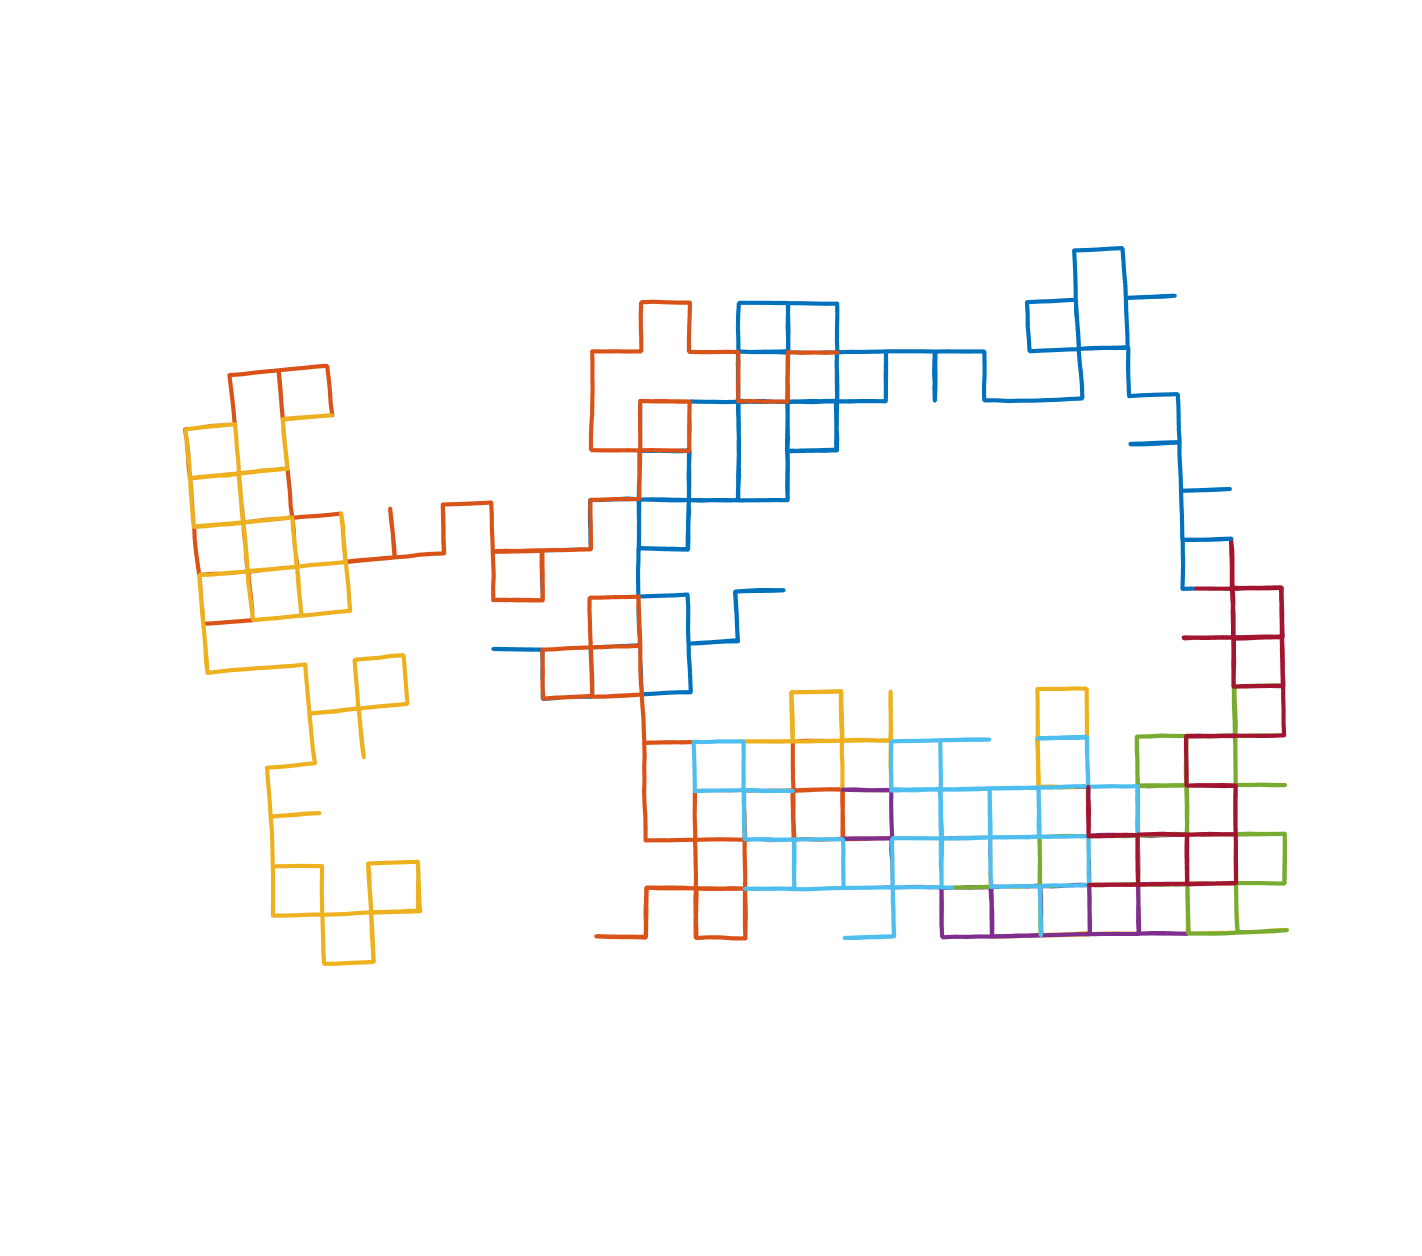
\includegraphics[trim =23mm 10mm 23mm 5mm,width=0.27\textwidth]{figures/benchmark/M3500.png}}&
		\hspace{1em}\subfloat[][\sf intel]{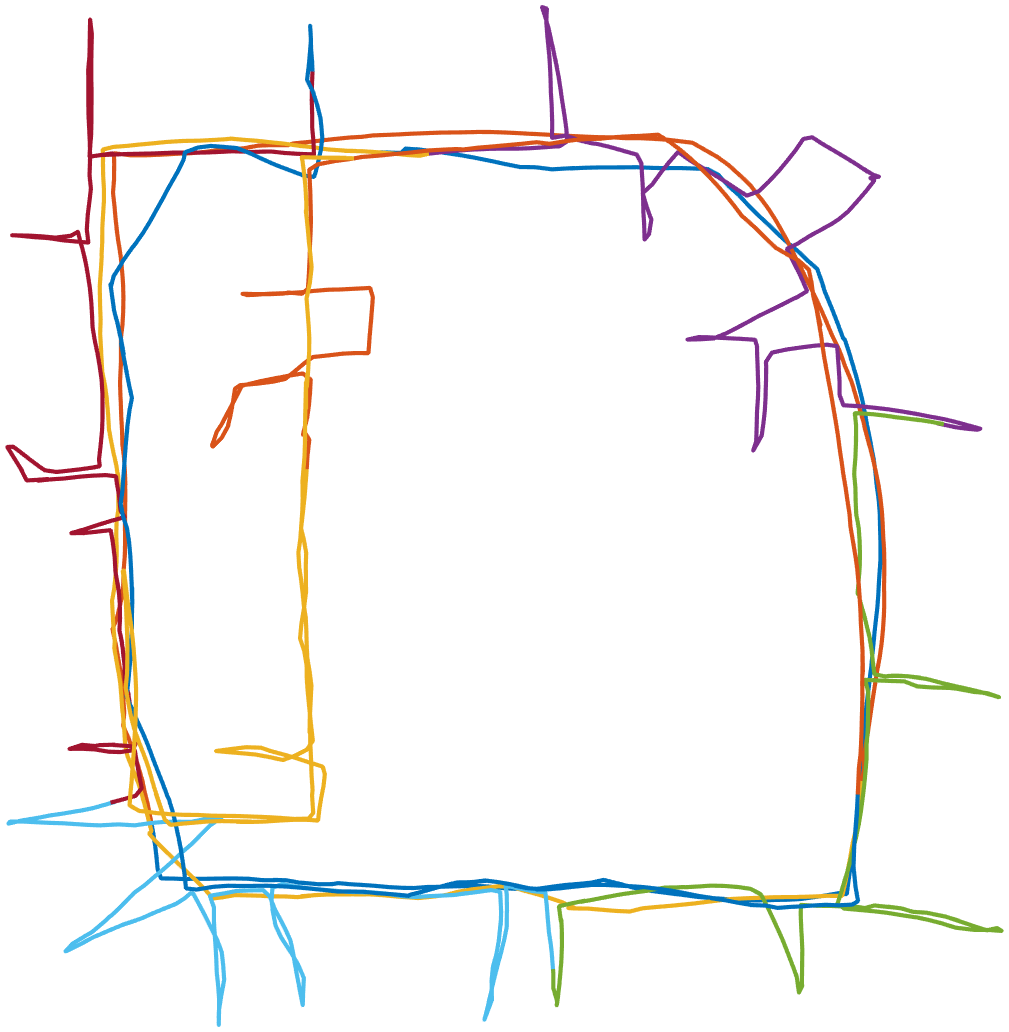
\includegraphics[trim =0mm 0mm 0mm 0mm,width=0.27\textwidth]{figures/benchmark/intel.png}}&
		\subfloat[][\sf MITb]{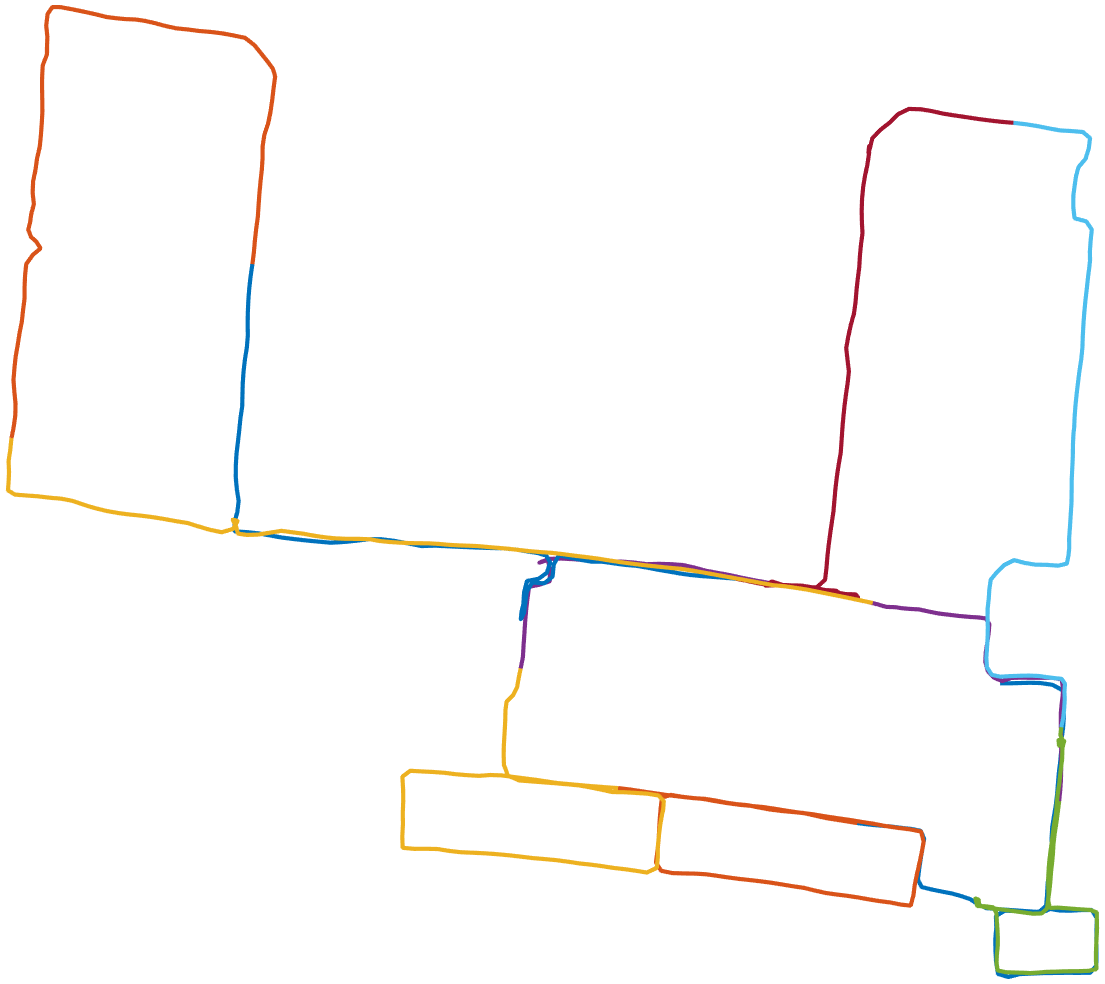
\includegraphics[trim =0mm 0mm 0mm 0mm,width=0.27\textwidth]{figures/benchmark/MITb.png}}
	\end{tabular}
	\caption{$\ammd$ results on the 2D SLAM benchmark datasets where the different colors denote the odometries of different robots. The distributed PGO has 10 robots  and is initialized with the distributed Nesterov's accelerated chordal initialization \cite{fan2020mm}. The number of iterations is 1000.}\label{fig::benchmark2D}
	\vspace{-0.25em}
	\centering
	\begin{tabular}{ccc}
		\subfloat[][\sf sphere]{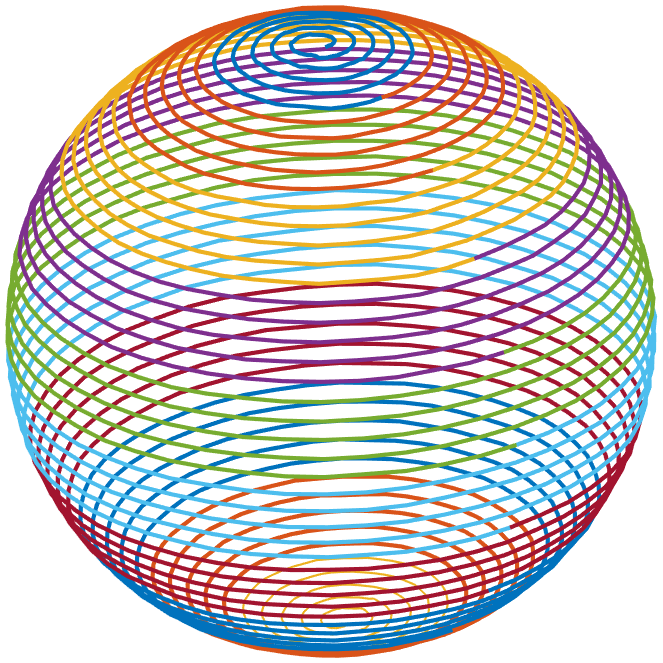
\includegraphics[trim =0mm 0mm 0mm 0mm,width=0.25\textwidth]{figures/benchmark/sphere2500.png}} &
		\subfloat[][\sf torus]{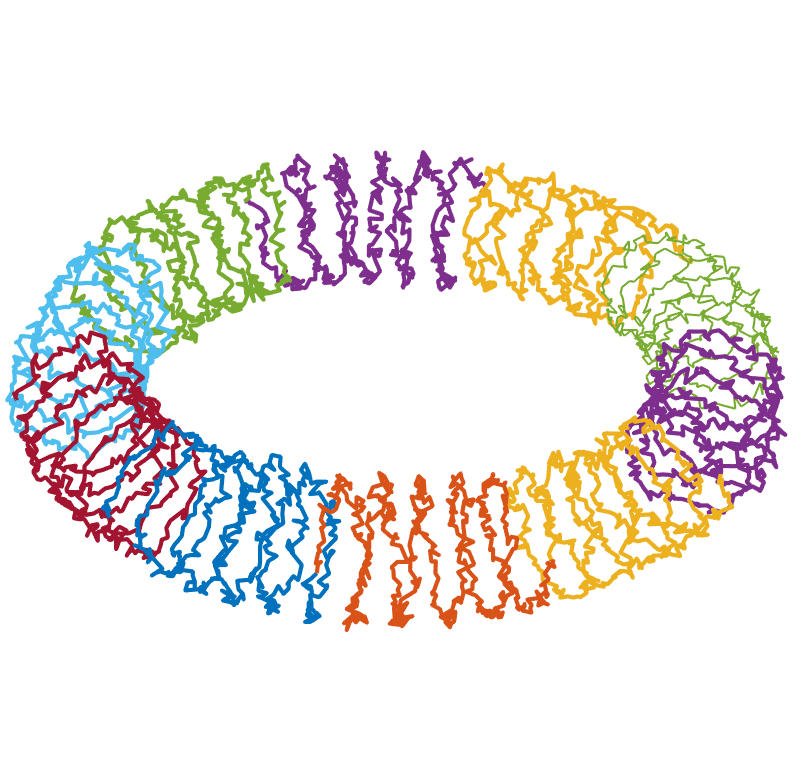
\includegraphics[trim =35mm 20mm 35mm 0mm,width=0.23\textwidth]{figures/benchmark/torus3D.png}} &
		\subfloat[][\sf grid]{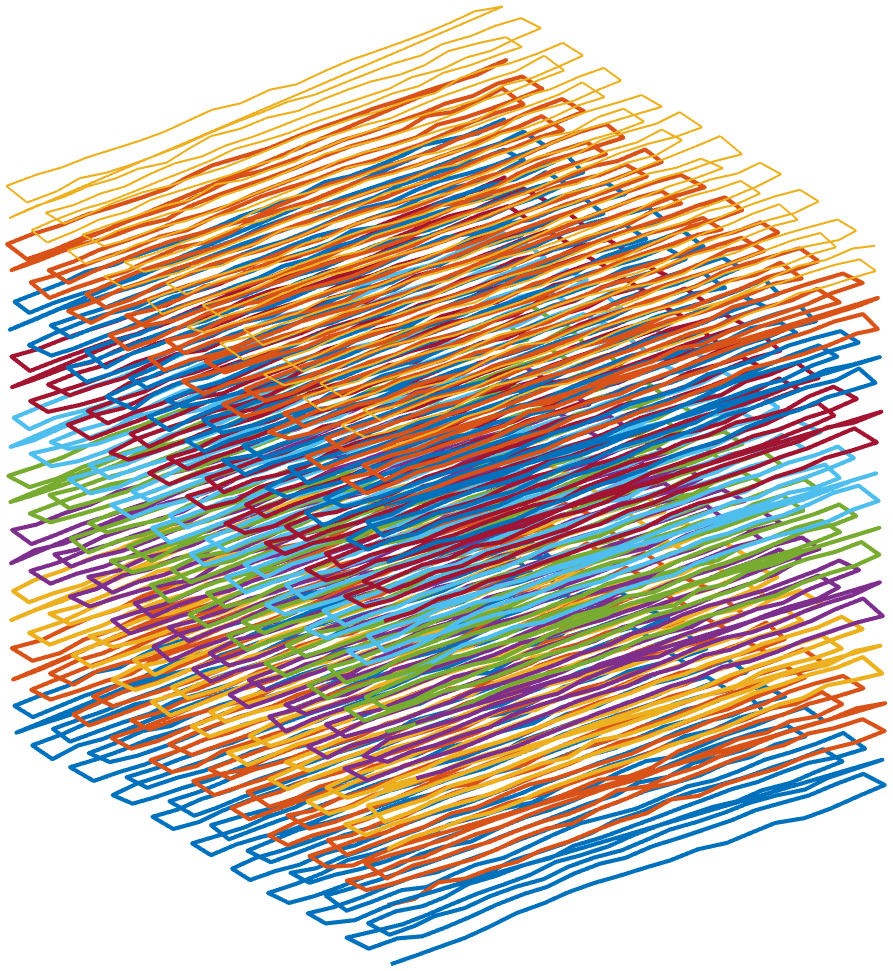
\includegraphics[trim =0mm 0mm 0mm 0mm,width=0.24\textwidth]{figures/benchmark/grid3D.png}}\\[1em]
		\subfloat[][\sf garage]{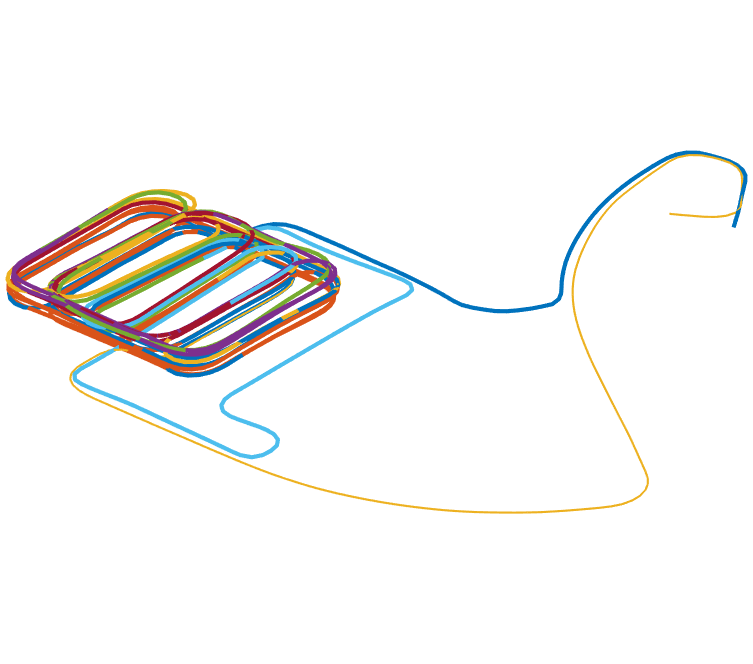
\includegraphics[trim =0mm 30mm 0mm 20mm,width=0.30\textwidth]{figures/benchmark/parking-garage.png}}&
		\subfloat[][\sf cubicle]{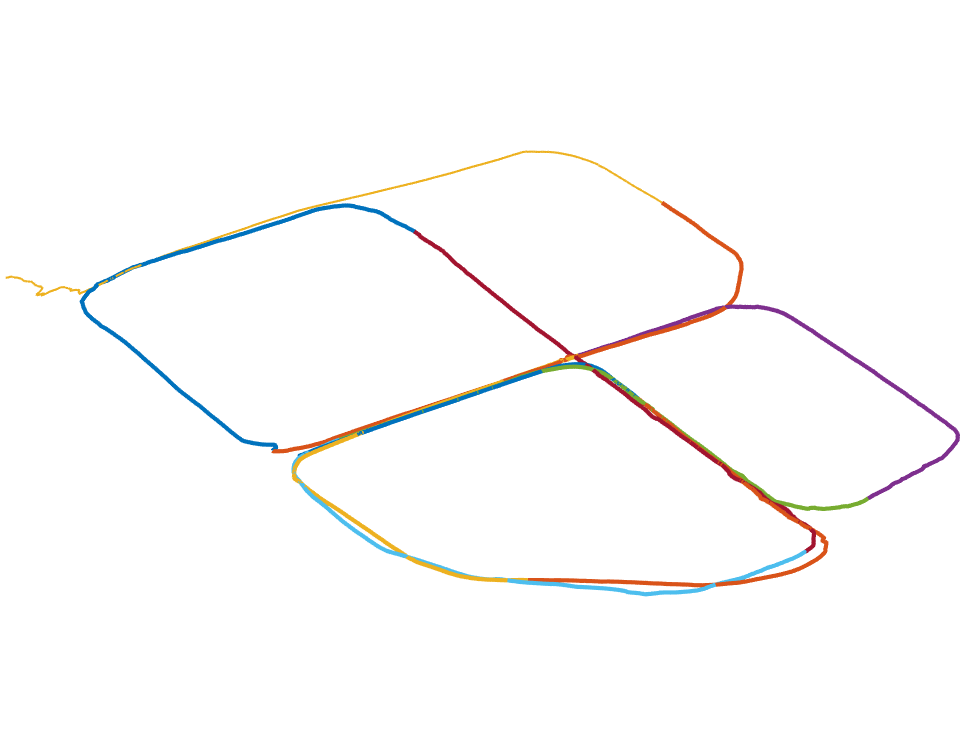
\includegraphics[trim =0mm 20mm 0mm 20mm,width=0.31\textwidth]{figures/benchmark/cubicle.png}}&
		\subfloat[][\sf rim]{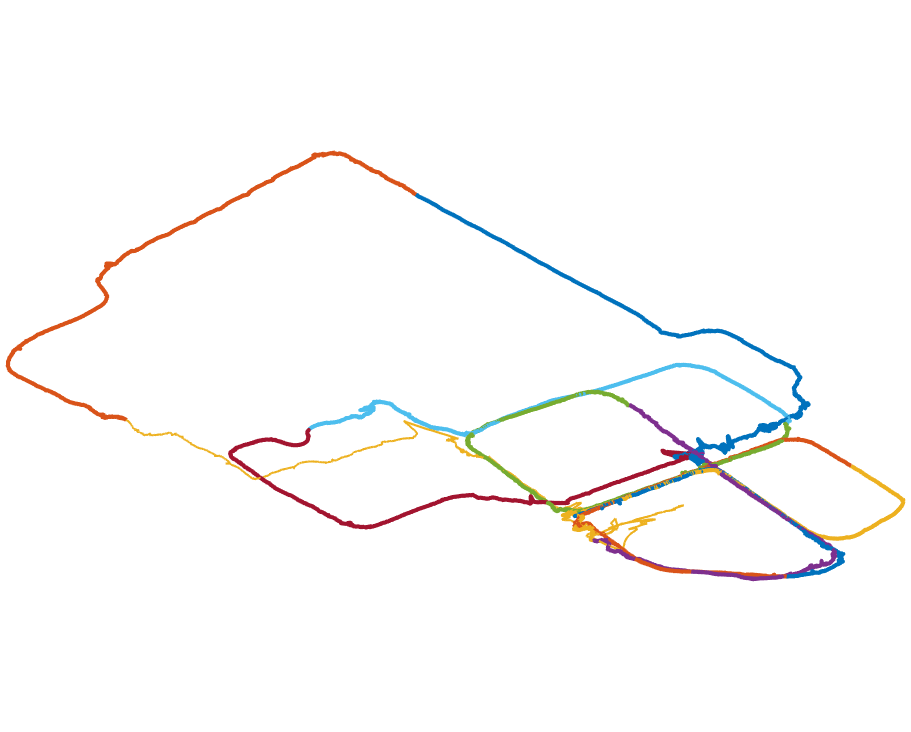
\includegraphics[trim =0mm 20mm 0mm 30mm,width=0.31\textwidth]{figures/benchmark/rim.png}}
	\end{tabular}
	\caption{$\ammd$ results on the 3D SLAM benchmark datasets where the different colors denote the odometries of different robots. The distributed PGO has 10 robots  and is initialized with the distributed Nesterov's accelerated chordal initialization \cite{fan2020mm}. The number of iterations is 1000.}\label{fig::benchmark3D}
	\vspace{-1.25em}
\end{figure*}